\section{Photon Map Generation}
We described in Chapter~\ref{chap:design} that the photon generation stage of the back end would run on multiple threads
to utilise the computing power of the machine the system is being run on, this required certain descitions to be made to
allow for the multiple threads to correclty distribute the power of the light sources into the scene.

Each thread is responsible for producing a certain proportion of the photons in the scene, once a thread has processed all
of these photons it will signal to the main thread that it has finished by sending a flag to the output queue the thread also
updates a global light emission count include the photons that the thread emitted for each of the lights, a seperate count for
each of the counts is kept as the processing of the threads may not happen at the same time.

\todo{Add the structure definition}

\subsection{Photon Emission}
In order to trace photons into the scene we first need a method of creating photons, this is implemented in the light 
defintion, each light object has a associated function that will produce a random photon from the light that is consitent with 
the type of light, for instance a point light will generate a photon with origin exactlu at the origin of the light source and
in a random direction, an area light produces a photon with origin on the area of the light with direction taken from a
cosine weighted hemisphere distribution in the direction of the normal of the light. Each photon that is emitted from the
light sources begin with the full power of the light source, this will be scaled by the number of emitted photons after
all photons have been gathered.

\subsection{Photon Tracing}
Once we have created a photon from a light source we now need to trace the photon through the scene and record the interactions
of the photon until it is absorbed or leaves the scene, the function that performes this function is \texttt{trace\_photon} the
declaration of this function is given below.

\texttt{int trace\_photon(scene\_t *scene, ray\_t *ray, int light, double power[3], bool specular, bool diffuse, bool specular\_only};

The parameters ray, light and power defines the photon properties, ray defines the origin and direction of the photon, light is an index
to the light from which this light was emited and the power contains the flux of the photon. specular and diffuse
define describe the path that the photons have taken prior to the call to \texttt{trace\_photon}

Photons are traced much like a ray in traditional raytracing, first we calculate the closest intersection point of the photon
once found the photon interacts with the surface of the object at the point of intersection this interaction can be specular 
reflection , transmission, diffuse reflection or absorbtion, at this point of intersection we must determine the path of the reflected
photon, the power of this photon is determined by the reflectance of the surface i.e a photon with white light that interacts with
a red surface will only reflect photons with power in the red component. Using the approach of scaling the photons will create a photon
map that correctly describes the distribution of power in the scene, unfortunatally this can lead to many photons with low power as they
are scaled at each interaction, it can also in the case of surfaces with both specualr and diffuse componenet lead to exponenetial number
of photons being produced as we need to create a reflected photon for both paths scaled apporoaprealty, as a result of these considerations

we have used a monte-carlo method that reflectes at most one photon
per surface interaction with full power, we ensure the correct result in the photon map by only reflecting the photon
with probability based on the reftance of the surface (i.e reflecting 50 full power photons as oppose to 100 full power photons)
we sample the reflectance of the surface by forming a cumulative distribution funciton of the materials reflectance coefficients.
Given the specular reflecive, transmissive and diffuse reflectance coefficents $\rho_{s}, \rho_{t}, \rho_{d}$
of the object we can create a cumulative distribution of photon emittion paths (Figure~\ref{fig:rr_dist}) 
we then take a uniform variable $\xi$ between 0 and 1 if the variable is within the distribution we reflect a photon, otherwise
the path of the photon is terminated. As we are using rgb values to store reflectance properties the
coeffients used to perform the sampling are the average of the three componenets, so as the distribution of the three
colour bands is correct we must also perform scaling of the power parameter that we use in the next \texttt{trace\_photon}
call, note that the scaling preserves the power of the photon and the reflectance properties of the surface.

\begin{figure}[h]
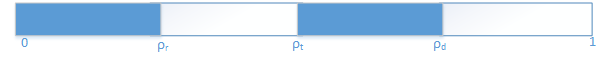
\includegraphics{./images/russian_roulette_distribution.png}
\label{fig:rr_dist}
\caption{Russian roulette distribution}
\end{figure}

At each non-specular interaction the photons are written to the output queue to be processed, this includes
the power of the photon, the incident angle of the photon to the surface and flags to indicate if the surface
has interacted with a diffuse or specular surface prior to this interaction, we do not store photon interactions
at specular surfaces as they do not provide us with information that can be used when estimating the radiance as
the probability of an incoming photon contributing to the specular reflectance is zero due to the delta functions
in the specular BRDF.

When creating the caustic photon map we are only concerned with those interactions with diffuse surfaces that have
taken a path that contains at least one specular bounce and no diffuse bounces (\textbf{LS$^+$DE}), as a result \texttt{trace\_photon}
has as input a flag that will indicate that any path that does not match this description should be discarded.

\subsubsection{Participating Media}
If the photon interacts with a participating medium the photon will begin a random walk inside the medium, the path of this walk
is determined by the properties of the medium, these being the scattering and absorbtion coefficient, the sum of which
is called the extinction coefficient, at each point in the random walk the photon is stored and then can either be
scattered or absorbed, the probability of being scattered is determined by the Albedo $\Lambda$

\missingfigure{random walk}

\begin{equation}
\Lambda = \frac{\sigma_s}{\sigma_e}
%\caption{Participating Media Albedo}
\end{equation}

The marching can be performed with a set distance and scaling of the photons at each step based on the attenuation of
light in participating media, a more efficient \cite{JensenBook} method is to importance sample the distance $\Delta x$ of the next interaction with 
Equation~\ref{eq:volume_dist_importance}, the scattering of the photon continues until the photon is absorbed, intersects
with an object in the medium or exits the medium. \todo{Expand the explination of this}

\begin{equation}
\Delta x = \frac{-log(\xi)}{\sigma_t(x)}
%\caption{Photon marching importance function}
\label{eq:volum_dist_importance}
\end{equation}

\subsection{Photon Processing}
The data from each photon emission thread is processed by a processing thread that reads the photons from the output queue
the photons will be places into a list bases upon the path that the photon took, for purly specular paths the photons
will be added to the caustinc photon map, for paths that end with an interaction with a participating media they will be
added to the volume photon map, all other paths are added to the global photon map. Once all photons have been collected
into the lists the main thread iterates over the photons and adjusts the photon power by the number of photons emitted by
the light that emitted the photon. \todo{clean up}

\subsection{K-D Tree Balancing (1 page)}
When performing radiance estimations with the photon map we will be performing nearest neighbour searches on points within
the map, this requires the photon map to be arrainged in a manner such that this search can be performed efficiently.
In order to do this we store the photon map in a left-balanced k-d tree. A left balanced tree is a tree structure where
at each level of the tree the depth of the children differs by at most one, \todo{finish the explination of the LEFT balanced tree}
this allows us to store the photon map in an array with the location of the children in the photon map known implicitly,
for a photon in position $i$ the children of the photon can be found at the $(2i + 1)^{th}$ and $(2i + 2)^{th}$
location for the left and right tree respectivly.

\begin{algorithm}
\begin{algorithmic}
\caption{Balanced K-D tree construction}
\Function{balance}{photons, index, max\_index}
\If
{
photons.size \textgreater 1
}
{
	\State axis $\gets$ \Call{select\_axis}{photons}
	\State left, median, right $\gets$ \Call{partition\_around\_median}{photons, axis}
	\State left\_index  $\gets$ 2 * index + 1
	\State right\_index $\gets$ 2 * index + 2

	\If{left\_index \textless max\_index}
		\State left $\gets$ \Call{balance}{left, left\_index,max\_index}
	\EndIf

	\If{right\_index \textless max\_index}
		\State right $\gets$ \Call{balance}{right, right\_index, max\_index}
	\EndIf

	\Return{left + median + right}
}
\Else
{

	\Return{photons}
}
\EndIf
\EndFunction
%\State colour $\gets$ scene.sky\_colour
%\For{object $\in$ scene}
%
%	new\_record $\gets$ intersects(ray, object)
%
%	\If{new\_record.hit \textbf{and} new\_record.t $\textless$ record.t}
%
%	record $\gets$ new\_record
%
%	\EndIf
%
%\EndFor
%
%\If{record.hit}
%
%	colour $\gets$ shade(scene, record)
%\EndIf
%
%\Return colour

\end{algorithmic}
\end{algorithm}

\begin{figure}
\centering
\begin{subfigure}{0.4\textwidth}
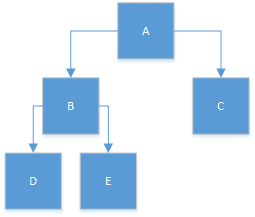
\includegraphics[scale=0.8]{./images/left-balanced-tree.png}
\caption{}
\end{subfigure}
\begin{subfigure}{0.4\textwidth}
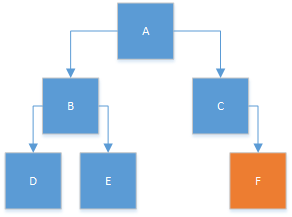
\includegraphics[scale=0.8]{./images/non-left-balanced-tree.png}
\caption{}
\end{subfigure}
\caption{(a) demonstrates a left balanced tree while (b) does not due to node F}
\end{figure}

\subsubsection{Selection Statistic}
During the balancing procedure we need to partition the tree such that half the elements are less than the median
this can be seen as finding the $i/2^{th}$ largest element in the list, this can be performed in linear time by using
the median of medians algorithm . Below is a comparison for the runnning time of the balancing procedure for
the nieve selection algorithm and the median of medians algorithm. As we are left-balancing the tree we also cannot
just take the median of the data, we must adjust the median such that the left half of the tree will fill before the right.
\todo{expand and add psuedocode}
